\section{A Simple And Interpretable Deep Gated  Network}
\begin{figure}[h]
\centering
\resizebox{0.6\columnwidth}{!}{
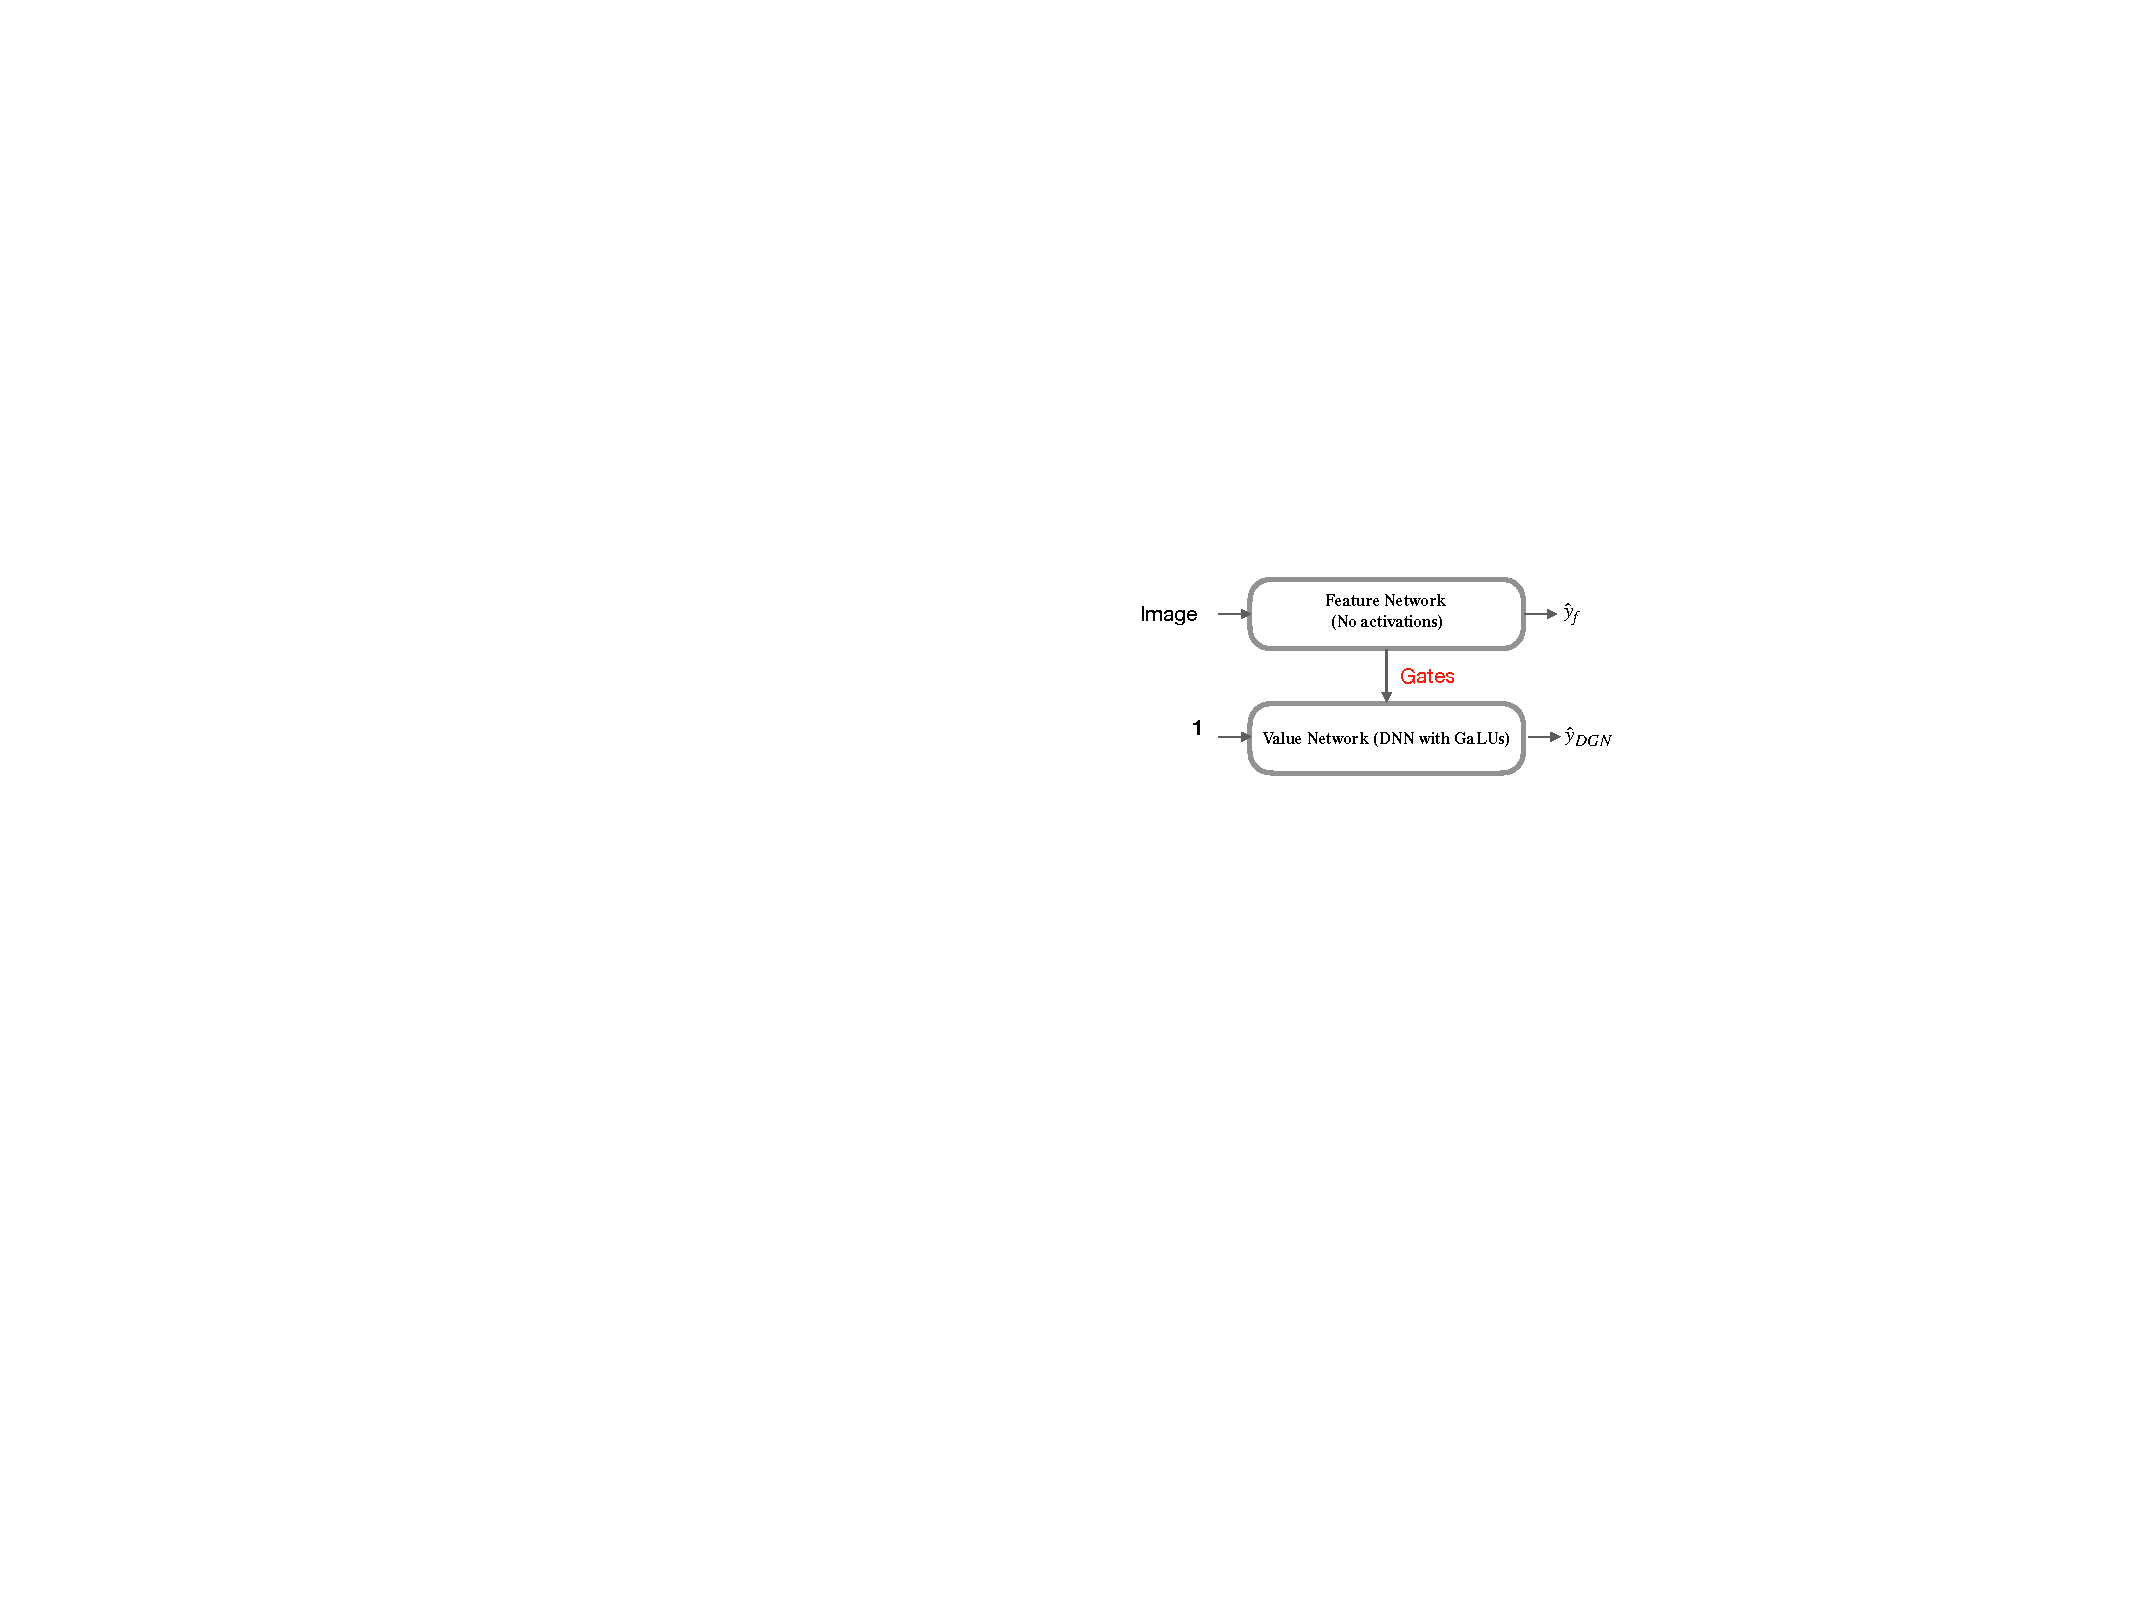
\includegraphics[scale=0.5]{figs/dgn-linear.pdf}
}
\end{figure}

\begin{comment}
\begin{wrapfigure}{r}{0.3\textwidth}
\resizebox{0.3\columnwidth}{!}{
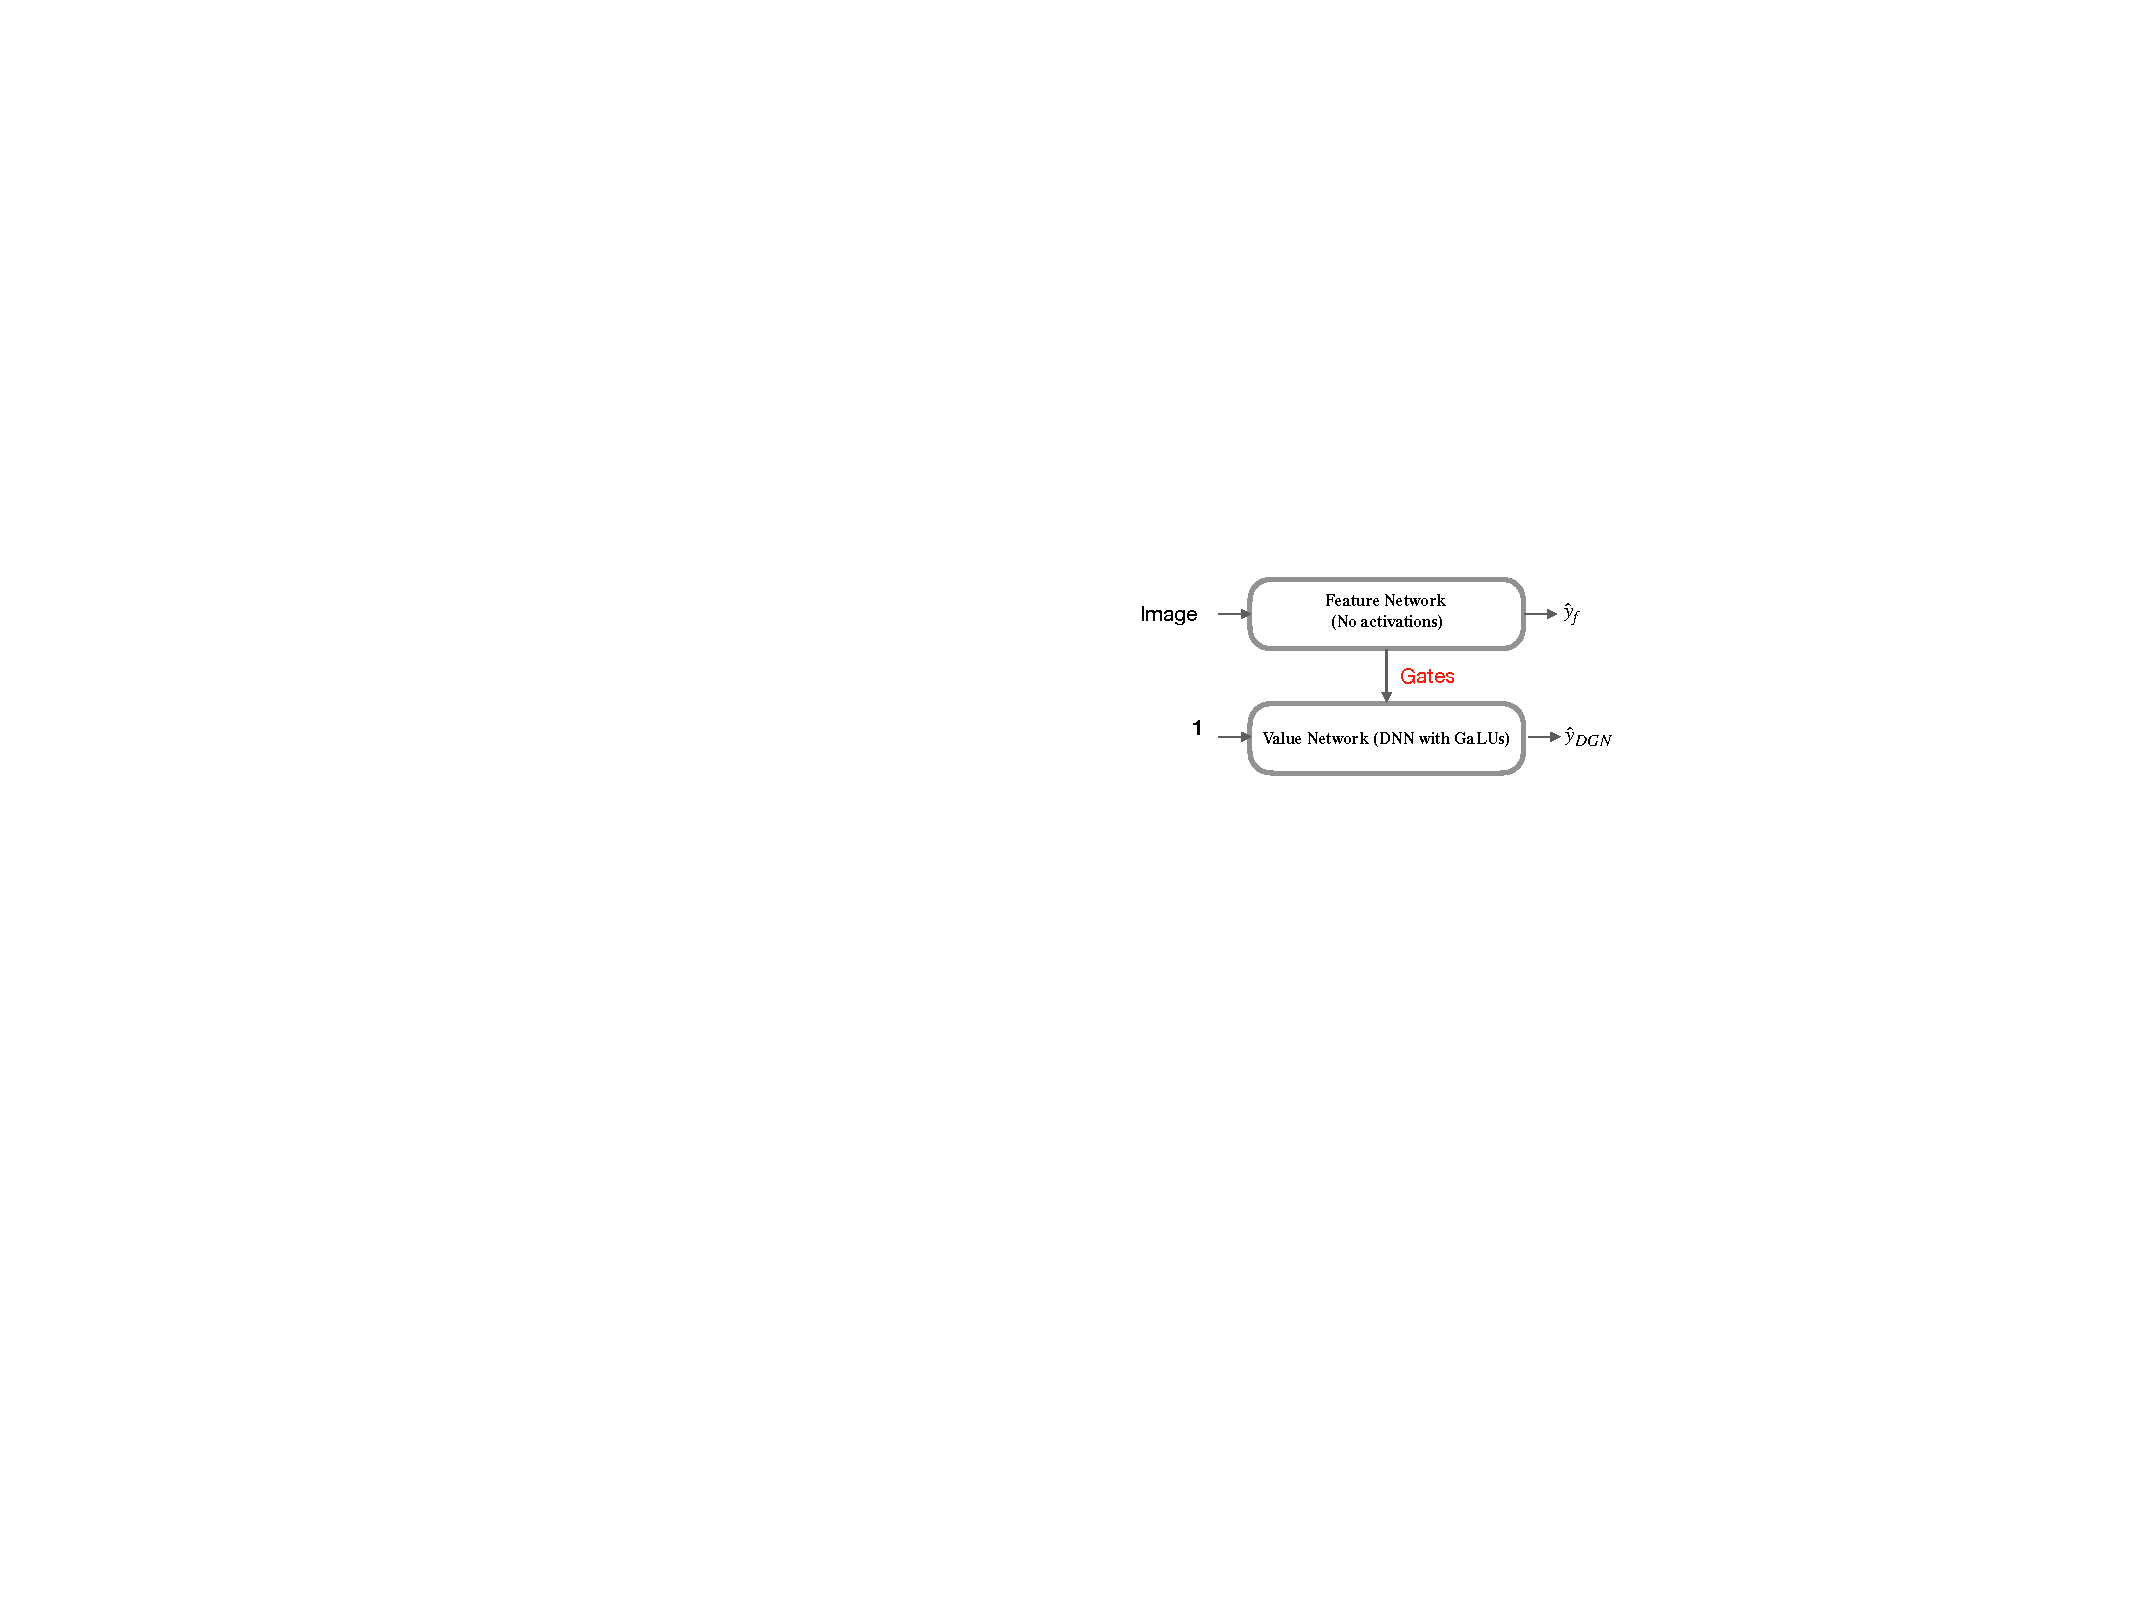
\includegraphics[scale=0.5]{figs/dgn-linear.pdf}
}
\end{wrapfigure}
\end{comment}
\textbf{Feature Network} is a fully linear network and comprises of $w$ convolutional windows in each layer. In order to make it simple, let us say tag the convolutional windows based on their `image processing' functionalities such as \emph{edge detection, sharpening, blurring} etc, and let us say that there are $K$ such functionalities. Let us denote these functionalities by operators $\F_1\ldots, \F_K$. For input $x\in\R^{\din}$ let us examine the outputs of various layers. Layer $1$ output has $\F_1\circ x ,\ldots, F_2\circ x$, and in layer $2$ output is given by $\F_i\circ\F_j x,i,j =1,\ldots,K$ and layer $d$ contains $\F_{i_d}\ldots\circ \F_{i_1} x, i_1,\ldots,i_d =1,\ldots,K$.  Note that we have used $\circ$ to denote composition of functionalities, however $\F_i\circ\F_j$ in the network it is indeed a multiplication of the weight matrices $\theta_a$ and $\theta_b$ ($a,b=1,\ldots,w$) which have functionalities $\F_i$ and $\F_j$. Thus the feature network can be completely understood in `image processing' functionalities and standard linear algebraic tools.

\textbf{Gating.} Each gate is triggered based on whether or not the layer input aligns with respect to the hyperplane given by the  incoming weights of the gate. The gates in a layer gives rise to the binary feature vector in the dimension equal to the number of gating units in that layer.

\textbf{Value Network}. Uses the gates from the feature network, lays them out depth-wise. From \Cref{th:mainconv} we know that in the limit of infinite width value network here implements the rotationally invariant NPK, and from the experimental results that the difference between finite and infinite width is in gate learning.

\textbf{Training and Testing.}
